% PAPER-001..005: one mathematical source for both languages.
\section{\lang{Bài toán và ký hiệu}{Problem definition and notation}}
\label{sec:problem}
\lang{Cho số nguyên $n\geq2$, đặt $N=n^2$. Sudoku là bảng $N\times N$ chia thành $N$ khối $n\times n$. Hàng và cột được đánh số từ 0; giá trị ô thuộc $D=\{1,\ldots,N\}$. Input dùng 0 cho ô trống. Một nghiệm điền đủ bảng, giữ các clues, và chứa mỗi giá trị đúng một lần trong từng hàng, cột và khối. Không yêu cầu nghiệm duy nhất.}{Let $n\geq2$ be an integer and $N=n^2$. The $N\times N$ Sudoku grid contains $N$ blocks of size $n\times n$. Rows and columns are zero-based; cell values belong to $D=\{1,\ldots,N\}$. Input uses 0 for an empty cell. A solution completes the grid, preserves its clues, and contains each value exactly once in every row, column, and block. Uniqueness is not required.}

\lang{Đặt $I=\{0,\ldots,N-1\}$, $J=\{0,\ldots,n-1\}$ và $G\subseteq I\times I\times D$ là tập các clue khác 0, với $g=|G|$. Biến Boolean $x_{r,c,v}$ đúng khi ô $(r,c)$ mang giá trị $v$. Có $N^3$ biến chính. Mapping của chương trình là}{Define $I=\{0,\ldots,N-1\}$, $J=\{0,\ldots,n-1\}$, and the nonzero clue triples $G\subseteq I\times I\times D$, with $g=|G|$. The Boolean variable $x_{r,c,v}$ is true exactly when cell $(r,c)$ contains value $v$. There are $N^3$ primary variables. The implementation maps them to}
\begin{equation}
 \operatorname{id}(r,c,v)=(rN+c)N+v\ \in\{1,\ldots,N^3\}.
\end{equation}
\lang{Parser từ chối cấu trúc/miền sai bằng INVALID\_INPUT. Clues mâu thuẫn nhưng đúng cấu trúc vẫn được mã hóa; tính không khả thi là UNSAT sau khi được chứng minh. Hình~\ref{fig:example4} minh họa $n=2$.}{The parser rejects malformed structure or domains as INVALID\_INPUT. Structurally valid conflicting clues are still encoded; infeasibility becomes UNSAT only when proved. Figure~\ref{fig:example4} illustrates $n=2$.}
% Constructed illustration, not a solver output or benchmark result.
\begin{figure}[pos=H]
\centering
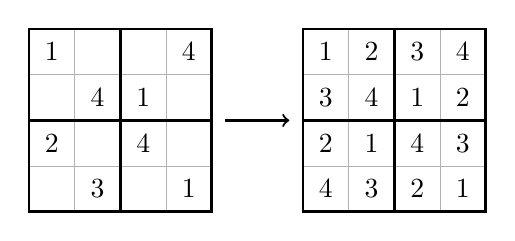
\begin{tikzpicture}[scale=0.58]
 \foreach \offset in {0,6} {
  \begin{scope}[xshift=\offset cm]
   \draw[step=1,gray!60,thin] (0,0) grid (4,4);
   \draw[line width=1pt] (0,0) rectangle (4,4);
   \draw[line width=1pt] (2,0)--(2,4) (0,2)--(4,2);
  \end{scope}
 }
 \foreach \x/\y/\v in {0/0/1,3/0/4,1/1/4,2/1/1,0/2/2,2/2/4,1/3/3,3/3/1}
  \node[text=black] at (\x+0.5,3.5-\y) {$\v$};
 \foreach \r/\vals in {0/{1,2,3,4},1/{3,4,1,2},2/{2,1,4,3},3/{4,3,2,1}}
  \foreach \v [count=\c from 0] in \vals
   \node[text=black] at (6.5+\c,3.5-\r) {$\v$};
 \draw[->,thick] (4.3,2)--(5.7,2);
\end{tikzpicture}
\caption{\lang{Ví dụ $4\times4$: input (trái) và một cách hoàn thành (phải) dựng để minh họa; không phải output solver hoặc chứng nhận uniqueness.}{A $4\times4$ input (left) and a constructed completion (right), for illustration; not solver output or a uniqueness certificate.}}
\label{fig:example4}
\end{figure}


\section{\lang{Mô hình SAT và ba AMO encoding}{SAT formulation and three AMO encodings}}
\label{sec:encoding}
\lang{Cách biểu diễn ô--giá trị và mô hình mở rộng của Lynce--Ouaknine là nền tảng tham khảo~\cite{lynce-ouaknine2006}. Với nhóm $Z=(z_1,\ldots,z_m)$, ràng buộc Exactly-One được tách thành ALO và AMO:}{The cell--value representation and extended formulation of Lynce--Ouaknine provide background~\cite{lynce-ouaknine2006}. For a group $Z=(z_1,\ldots,z_m)$, Exactly-One decomposes into ALO and AMO:}
\begin{equation}
 \operatorname{EXO}(Z)=\operatorname{ALO}(Z)\land\operatorname{AMO}(Z),
 \qquad\operatorname{ALO}(Z)=\bigvee_{i=1}^{m}z_i.
\end{equation}
\lang{Bốn họ sau, mỗi họ có $N^2$ nhóm dài $N$, cùng các clue unit clauses tạo công thức Sudoku:}{The following four families each contain $N^2$ groups of length $N$. Together with the clue units they form the Sudoku formula:}
\begin{align}
 &\bigwedge_{r,c\in I}\operatorname{EXO}\{x_{r,c,v}:v\in D\}, &&\lang{\text{ô}}{\text{cell}};\label{eq:cell}\\
 &\bigwedge_{r\in I,v\in D}\operatorname{EXO}\{x_{r,c,v}:c\in I\}, &&\lang{\text{hàng--giá trị}}{\text{row--value}};\\
 &\bigwedge_{c\in I,v\in D}\operatorname{EXO}\{x_{r,c,v}:r\in I\}, &&\lang{\text{cột--giá trị}}{\text{column--value}};\\
 &\bigwedge_{p,q\in J,v\in D}\operatorname{EXO}\{x_{pn+u,qn+w,v}:u,w\in J\}, &&\lang{\text{khối--giá trị}}{\text{block--value}};\label{eq:block}\\
 &\bigwedge_{(r,c,v)\in G}x_{r,c,v}, &&\lang{\text{clues}}{\text{clues}}.\label{eq:clues}
\end{align}
\lang{Như vậy có $4N^2$ nhóm EXO. Code sinh cùng thứ tự nhóm/literal cho mọi encoder; mỗi nhóm thêm ALO trước AMO, cuối cùng thêm clues theo hàng. Không loại clause trùng, không symmetry breaking hay tiền xử lý riêng theo clue.}{Thus there are $4N^2$ EXO groups. Code uses the same group/literal order for every encoder, appends ALO before AMO within each group, and then appends clues in row-major order. Duplicate clauses remain; no symmetry breaking or clue-specific preprocessing is applied.}

\subsection{Pairwise}
\begin{equation}
 E_{\rm pw}(Z)=\bigwedge_{1\leq i<j\leq m}(\neg z_i\lor\neg z_j).
\end{equation}
\lang{Mọi cặp input không được cùng đúng. Code tạo trực tiếp các cặp, không dùng biến phụ.}{Every input pair is forbidden from being simultaneously true. Code generates these pairs directly without auxiliaries.}

\subsection{Sequential counter}
\lang{Theo nguyên lý sequential unary counter~\cite{sinz2005}, có thể đặc tả AMO bằng chuỗi $s_1,\ldots,s_{m-1}$:}{Following the sequential unary counter principle~\cite{sinz2005}, AMO can be specified using a chain $s_1,\ldots,s_{m-1}$:}
\begin{align}
 E_{\rm sc}(Z,S)={}&(\neg z_1\lor s_1)\land(\neg z_m\lor\neg s_{m-1})\notag\\
 &{}\land\bigwedge_{i=2}^{m-1}
 \bigl[(\neg z_i\lor s_i)\land(\neg s_{i-1}\lor s_i)
       \land(\neg z_i\lor\neg s_{i-1})\bigr].
\end{align}
\lang{Input đúng làm chuỗi truyền về sau, ngăn một input sau đó cũng đúng. Chiều mở rộng chọn $s_i=\bigvee_{j\leq i}z_j$. Chương trình gọi \texttt{CardEnc.atmost} với \texttt{bound=1}, \texttt{EncType.seqcounter} và \texttt{top\_id} hiện hành~\cite{pysat-card,pysat2018}. Biểu thức trên mô tả nguyên lý/semantics, không khẳng định thứ tự literal hay biến phụ trùng nguyên byte với binary PySAT.}{A true input propagates along the chain, excluding any later true input. For an extension, choose $s_i=\bigvee_{j\leq i}z_j$. The program calls \texttt{CardEnc.atmost} with \texttt{bound=1}, \texttt{EncType.seqcounter}, and the current \texttt{top\_id}~\cite{pysat-card,pysat2018}. The expression specifies the principle and semantics; it does not claim byte-for-byte literal order or auxiliary naming in the PySAT binary.}

\subsection{Bitwise AMO}
\lang{Đặt $k=\lceil\log_2m\rceil$ và gán mỗi input một mã nhị phân khác nhau $b(i)\in\{0,1\}^k$. Với các selector $a_1,\ldots,a_k$, đặt $\ell_{ij}=a_j$ nếu $b(i)_j=1$, và $\ell_{ij}=\neg a_j$ nếu $b(i)_j=0$. Khi đó}{Let $k=\lceil\log_2m\rceil$ and assign each input a distinct binary code $b(i)\in\{0,1\}^k$. With selectors $a_1,\ldots,a_k$, let $\ell_{ij}=a_j$ if $b(i)_j=1$, and $\ell_{ij}=\neg a_j$ otherwise. Then}
\begin{equation}
 E_{\rm bw}(Z,A)=\bigwedge_{i=1}^{m}\bigwedge_{j=1}^{k}(\neg z_i\lor\ell_{ij}).
\end{equation}
\lang{Hai input đúng đòi hai mã khác nhau nên xung đột ở ít nhất một bit. Khi có một input đúng, chọn mã của nó; khi không có input đúng, chọn selector tùy ý. Chương trình dùng \texttt{EncType.bitwise} qua cùng API AMO. Đây là mã hóa AMO cho các literal one-hot, không phải thay biến ô bằng số nhị phân. Nguồn API/source bitwise được ghi riêng~\cite{pysat-card,pysat-bitwise-source}; không gán encoding này cho Sinz.}{Two true inputs require distinct codes and therefore conflict on at least one bit. With one true input, choose its code; with no true inputs, selectors are arbitrary. The program uses \texttt{EncType.bitwise} through the same AMO API. This encodes AMO over one-hot literals; it does not replace Sudoku cell variables by binary numbers. The bitwise API/source is credited separately~\cite{pysat-card,pysat-bitwise-source}, not attributed to Sinz.}

\section{\lang{Tính đúng đắn}{Correctness}}
\lang{Gọi $F_e(X,A)$ là CNF cho encoding $e$, gồm cả clues. Mỗi AMO phải thỏa đặc tả $\exists A_Z\,E_e(Z,A_Z)\iff\sum_i z_i\leq1$. Các cấu trúc trên đáp ứng đặc tả này. Trong code, toàn bộ $N^3$ ID chính được dự trữ trước; mỗi nhóm cấp biến phụ phía trên \texttt{top\_id} và cập nhật nó, nên các nhóm không dùng chung biến phụ. Khi đó}{Let $F_e(X,A)$ be the CNF for encoding $e$, including clues. Each AMO must satisfy $\exists A_Z\,E_e(Z,A_Z)\iff\sum_i z_i\leq1$, as the constructions above do. Code reserves all $N^3$ primary IDs first, allocates each group's auxiliaries above \texttt{top\_id}, and updates it, so groups do not share auxiliaries. Thus}
\begin{equation}
 \exists A\,F_e(X,A)\quad\Longleftrightarrow\quad
 \operatorname{Sudoku}_G(X).
\end{equation}
\lang{\textbf{Chiều thuận.} ALO và AMO của ô cho đúng một giá trị trong mỗi ô. Các nhóm hàng--giá trị, cột--giá trị và khối--giá trị cho mỗi giá trị xuất hiện đúng một lần trong các đơn vị tương ứng. Unit clauses giữ mọi clue. Vì vậy giải mã các biến chính của một model CNF tạo một nghiệm hợp lệ.}{\textbf{Forward direction.} Cell ALO and AMO give exactly one value per cell. Row--value, column--value, and block--value groups require every value exactly once in the corresponding unit. Unit clauses preserve every clue. Decoding a CNF model's primary variables therefore yields a valid solution.}

\lang{\textbf{Chiều ngược.} Từ một nghiệm Sudoku giữ clues, đặt đúng các biến ô--giá trị được chọn; mỗi nhóm có đúng một input đúng. Pairwise đã thỏa; sequential mở rộng bằng các OR tiền tố; bitwise chọn mã input đúng. Do các nhóm có tập phụ rời nhau, ghép các mở rộng cục bộ thành một phép gán $A$ thỏa toàn CNF. Không đòi mọi phép gán phụ đều thỏa, cũng không suy nghiệm là duy nhất.}{\textbf{Reverse direction.} From a Sudoku solution preserving clues, set the selected cell--value variables true. Every group has exactly one true input. Pairwise is already satisfied; extend sequential groups by prefix ORs and bitwise groups by the true input's code. Disjoint auxiliary sets let these local extensions combine into a global satisfying assignment $A$. This does not require every auxiliary assignment to satisfy the CNF, nor imply uniqueness.}

\section{\lang{Kích thước lý thuyết và số đếm đã kiểm}{Theoretical size and checked counts}}
\label{sec:counts}
\lang{Với $m\geq4$, các cấu trúc AMO được trình bày có số phụ $a_e(m)$ và clause $c_e(m)$ như sau:}{For $m\geq4$, the presented AMO constructions have the following auxiliary counts $a_e(m)$ and clause counts $c_e(m)$:}
\begin{equation}
\begin{array}{c|cc}
 e & a_e(m)&c_e(m)\\\hline
 \mathrm{pairwise}&0&m(m-1)/2\\
 \mathrm{seqcounter}&m-1&3m-4\\
 \mathrm{bitwise}&\lceil\log_2m\rceil&m\lceil\log_2m\rceil
\end{array}
\end{equation}
\lang{Do mỗi nhóm còn một ALO, tổng lý thuyết là}{Including one ALO per group, the theoretical totals are}
\begin{equation}
 V_e=N^3+4N^2a_e(N),\qquad
 C_e=4N^2[1+c_e(N)]+g.
\end{equation}
\lang{Pairwise có chính xác $N^3$ biến và $4N^2[1+N(N-1)/2]+g$ clause khi giữ trùng. Các cấu trúc cho độ lớn clause lần lượt $\Theta(N^4)$, $\Theta(N^3)$, $\Theta(N^3\log N)$; cả ba có tổng biến $\Theta(N^3)$, vì $g\leq N^2$. Đây là kích thước biểu diễn, không phải giới hạn thời gian solve hoặc bằng chứng encoder nào nhanh hơn.}{Pairwise has exactly $N^3$ variables and $4N^2[1+N(N-1)/2]+g$ clauses with duplicates retained. Clause growth for the constructions is respectively $\Theta(N^4)$, $\Theta(N^3)$, and $\Theta(N^3\log N)$; all have $\Theta(N^3)$ total variables, since $g\leq N^2$. These describe representation size, not solve-time bounds or evidence of a faster encoder.}

\lang{Bảng~\ref{tab:cnf-counts} được sinh từ \texttt{diagnostics/model/results.json}: PySAT 1.9.dev16, $N\in\{4,9,16,25\}$. Đây là số đếm CNF trước preprocessing, không phải benchmark; các ca chẩn đoán có $g=2$ và bảng trừ hai clue unit để hiển thị $C-g$. Seqcounter/bitwise quan sát được khớp các biểu thức trên tại bốn kích thước này. Không suy mọi biến thể/thư viện hay mọi độ dài input có cùng count; API có thể có shortcut ở nhóm nhỏ. Source upstream đã đọc chưa được coi là bằng chứng binary đang chạy.}{Table~\ref{tab:cnf-counts} is generated from \texttt{diagnostics/model/results.json}: PySAT 1.9.dev16, $N\in\{4,9,16,25\}$. These are pre-preprocessing CNF counts, not benchmarks. Diagnostic cases have $g=2$; the table subtracts the two clue units to show $C-g$. Observed seqcounter/bitwise counts match the expressions at these four sizes. This does not assert identical counts for every variant, library, or input length; small groups may use API shortcuts. The upstream source read is not treated as proof of the running binary.}
% Generated by export_model_counts.py; do not edit counts by hand.
\begin{table}[pos=H]
\centering
\caption{\lang{Số đếm cấu trúc từ diagnostics; $C-g$ không gồm clue units.}{Structural counts from diagnostics; $C-g$ excludes clue units.}}
\label{tab:cnf-counts}
\begin{tabular}{rlrrrr}
\toprule
$N$ & AMO & $N^3$ & \lang{Phụ}{Aux.} & $V_e$ & $C_e-g$\\
\midrule
4 & pairwise & 64 & 0 & 64 & 448\\
4 & seqcounter & 64 & 192 & 256 & 576\\
4 & bitwise & 64 & 128 & 192 & 576\\
9 & pairwise & 729 & 0 & 729 & 11988\\
9 & seqcounter & 729 & 2592 & 3321 & 7776\\
9 & bitwise & 729 & 1296 & 2025 & 11988\\
16 & pairwise & 4096 & 0 & 4096 & 123904\\
16 & seqcounter & 4096 & 15360 & 19456 & 46080\\
16 & bitwise & 4096 & 4096 & 8192 & 66560\\
25 & pairwise & 15625 & 0 & 15625 & 752500\\
25 & seqcounter & 15625 & 60000 & 75625 & 180000\\
25 & bitwise & 15625 & 12500 & 28125 & 315000\\
\bottomrule
\end{tabular}
\end{table}

